\documentclass[12pt,a4paper]{article}
\usepackage[marginparsep=8pt,left=2.5cm,right=2.5cm,top=2.5cm,bottom=3cm]{geometry}
\usepackage{graphicx}
\usepackage[utf8]{inputenc}
\usepackage{amsmath}
%\setlength{\parindent}{0pt}% Remove paragraph indent
\graphicspath{ {./images/} }
\newcommand*\rfrac[2]{{}^{#1}\!/_{#2}}

\newcommand{\overbar}[1]{\mkern 2.5mu\overline{\mkern-2.5mu#1\mkern-2.5mu}\mkern 2.5mu}

\begin{document}

\title{\LARGE \bf Domácí úkol na BI-PST 2018}
 \author{Pavel Jahoda a Jan Lidák}

\maketitle

\section{Úkol 1}
Data jsou z pozorování 59 vrabců během zimy. První veličina {\bf X} reprezentuje váhy vrabců v gramech. Druhá veličina {\bf Y} nabývá dvou hodnot 'survived', pokud vrabec přežil a 'perished' pokud nepřežil. Sledovanou proměnnou X jsme rozdělili na dvě pozorované skupiny {\bf X1} (vrabci co přežili) a {\bf X2} (vrabci co nepřežili).\\
EX1=25.463, var(X1)=1.539 a medián je 25.7.\\
EX1=26.275, var(X2)=2.078 a medián je 26.\\
\par \bigskip

\section{Úkol 2}
Nejprve vykreslíme histogram a graf empirické distribuční funkce pro vrabce kteří přežili. 
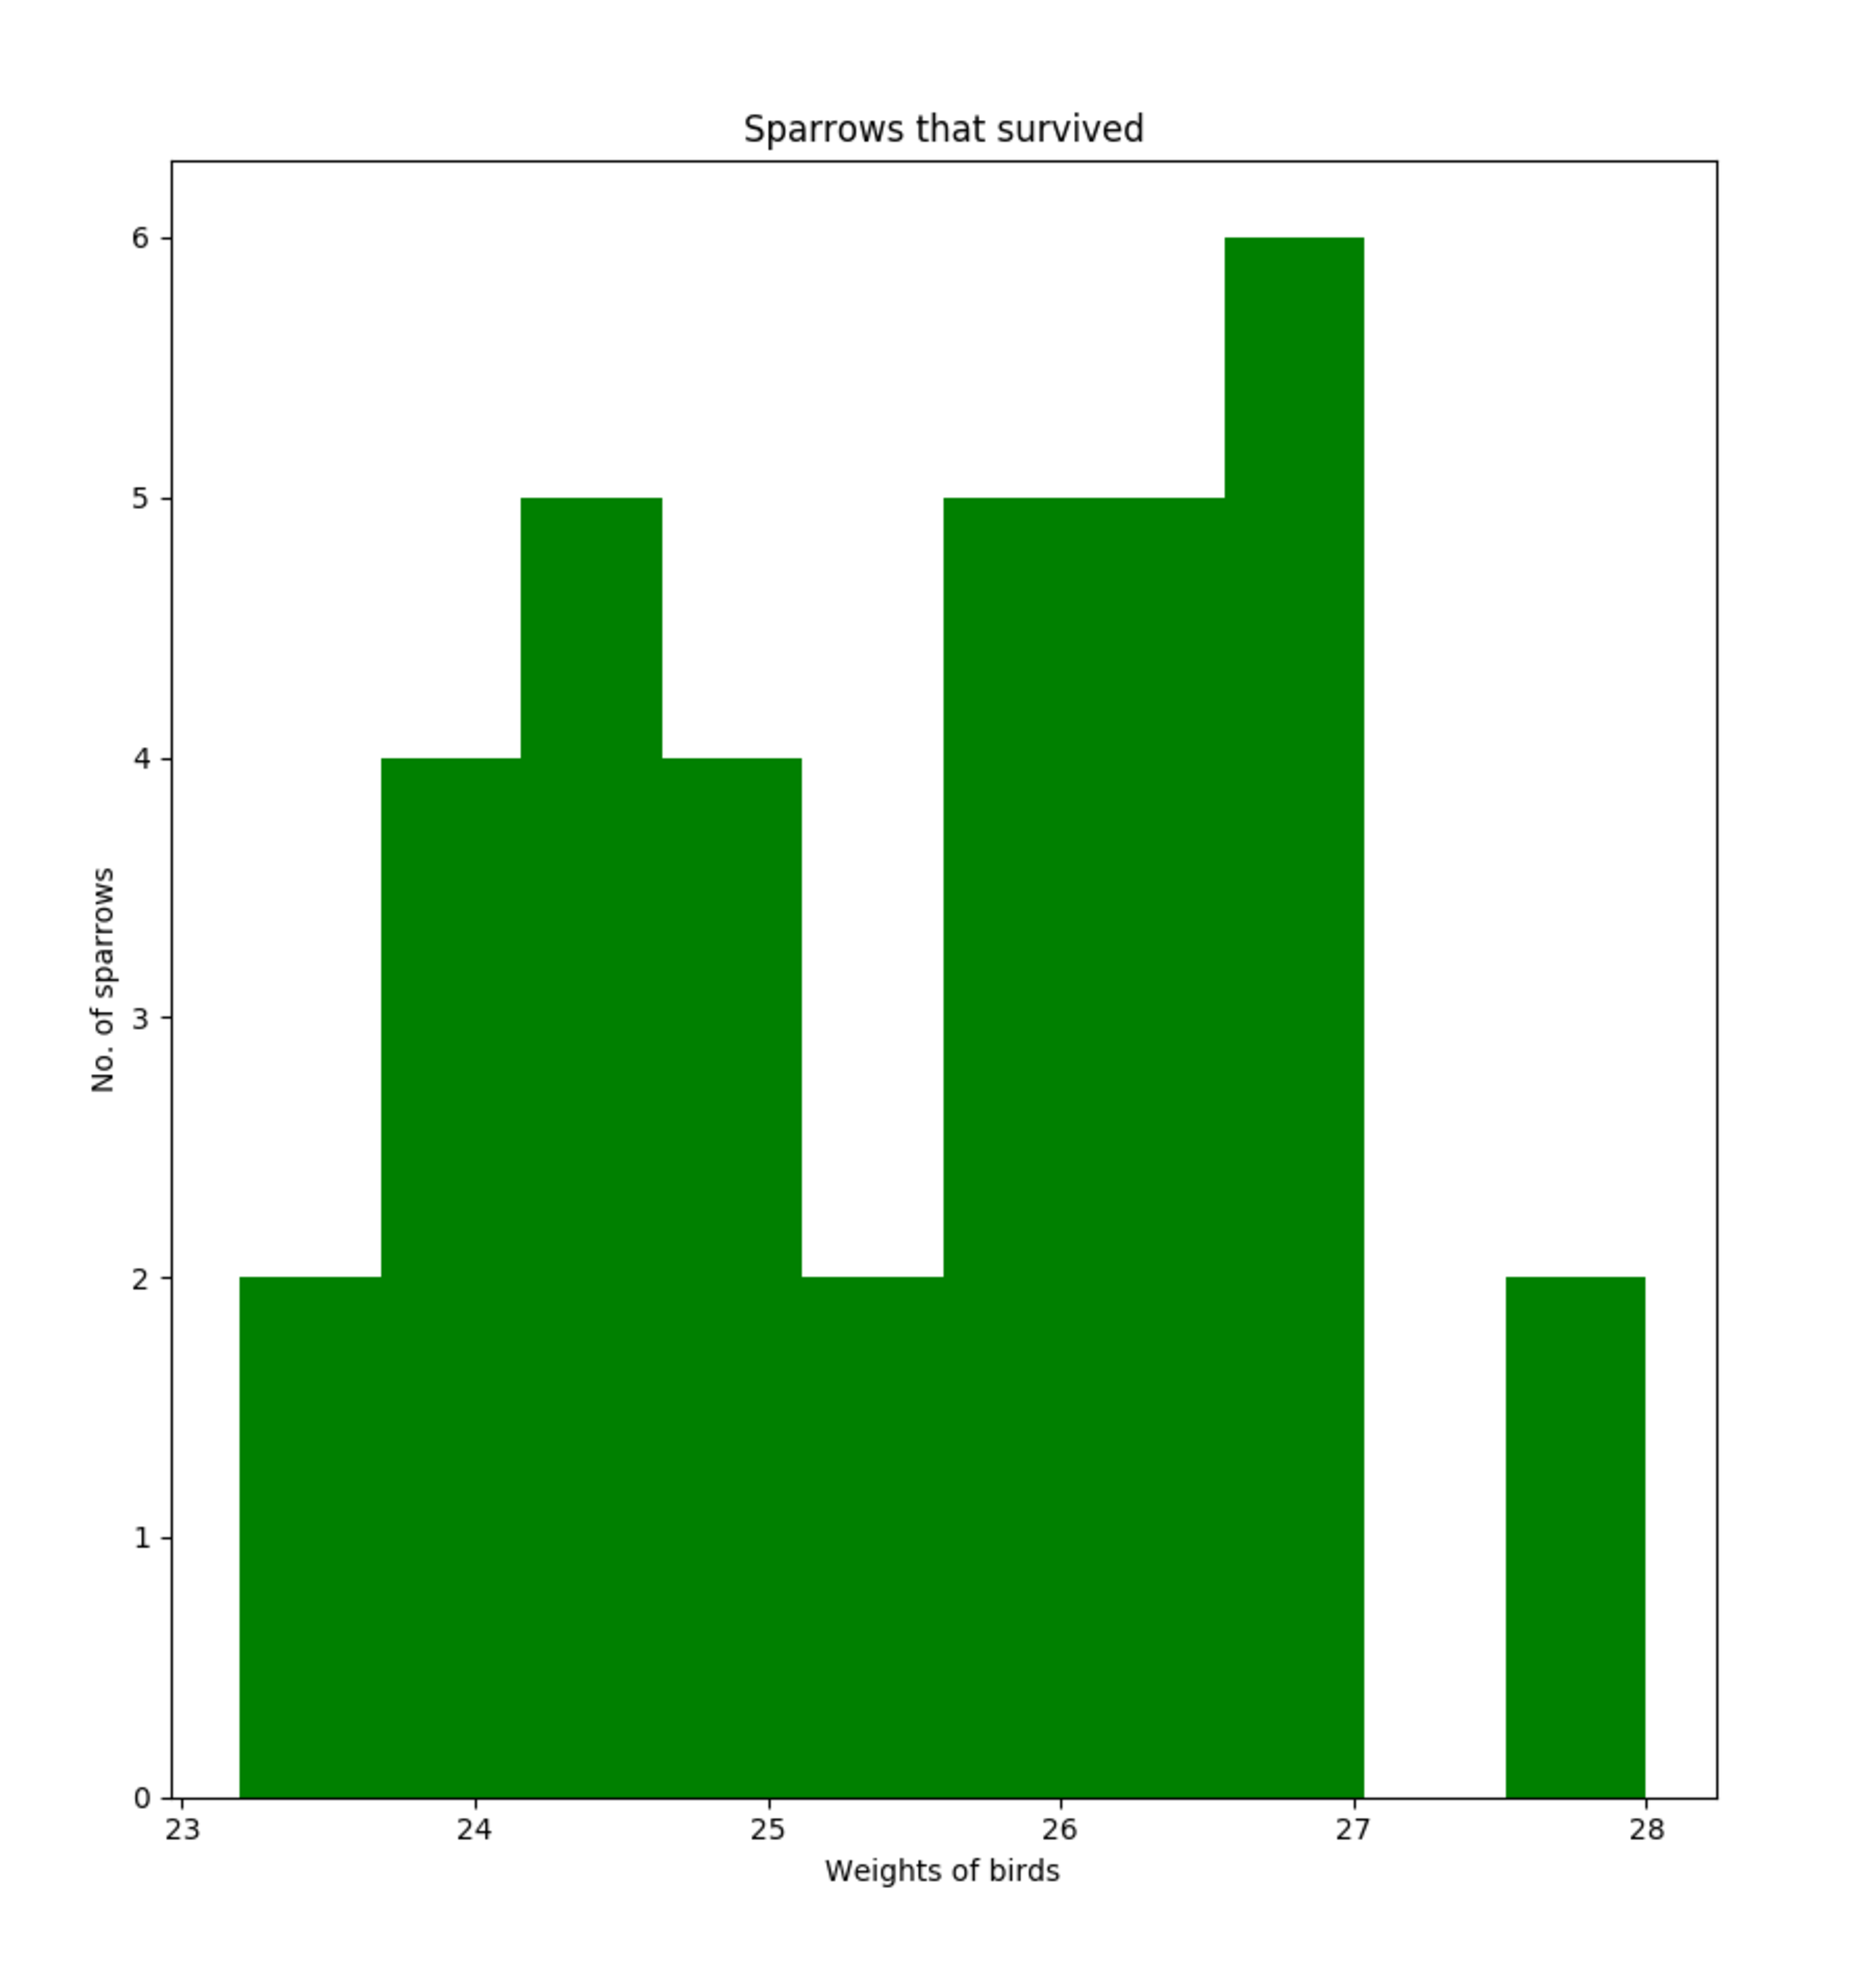
\includegraphics[height=3.5in]{survivedHist}
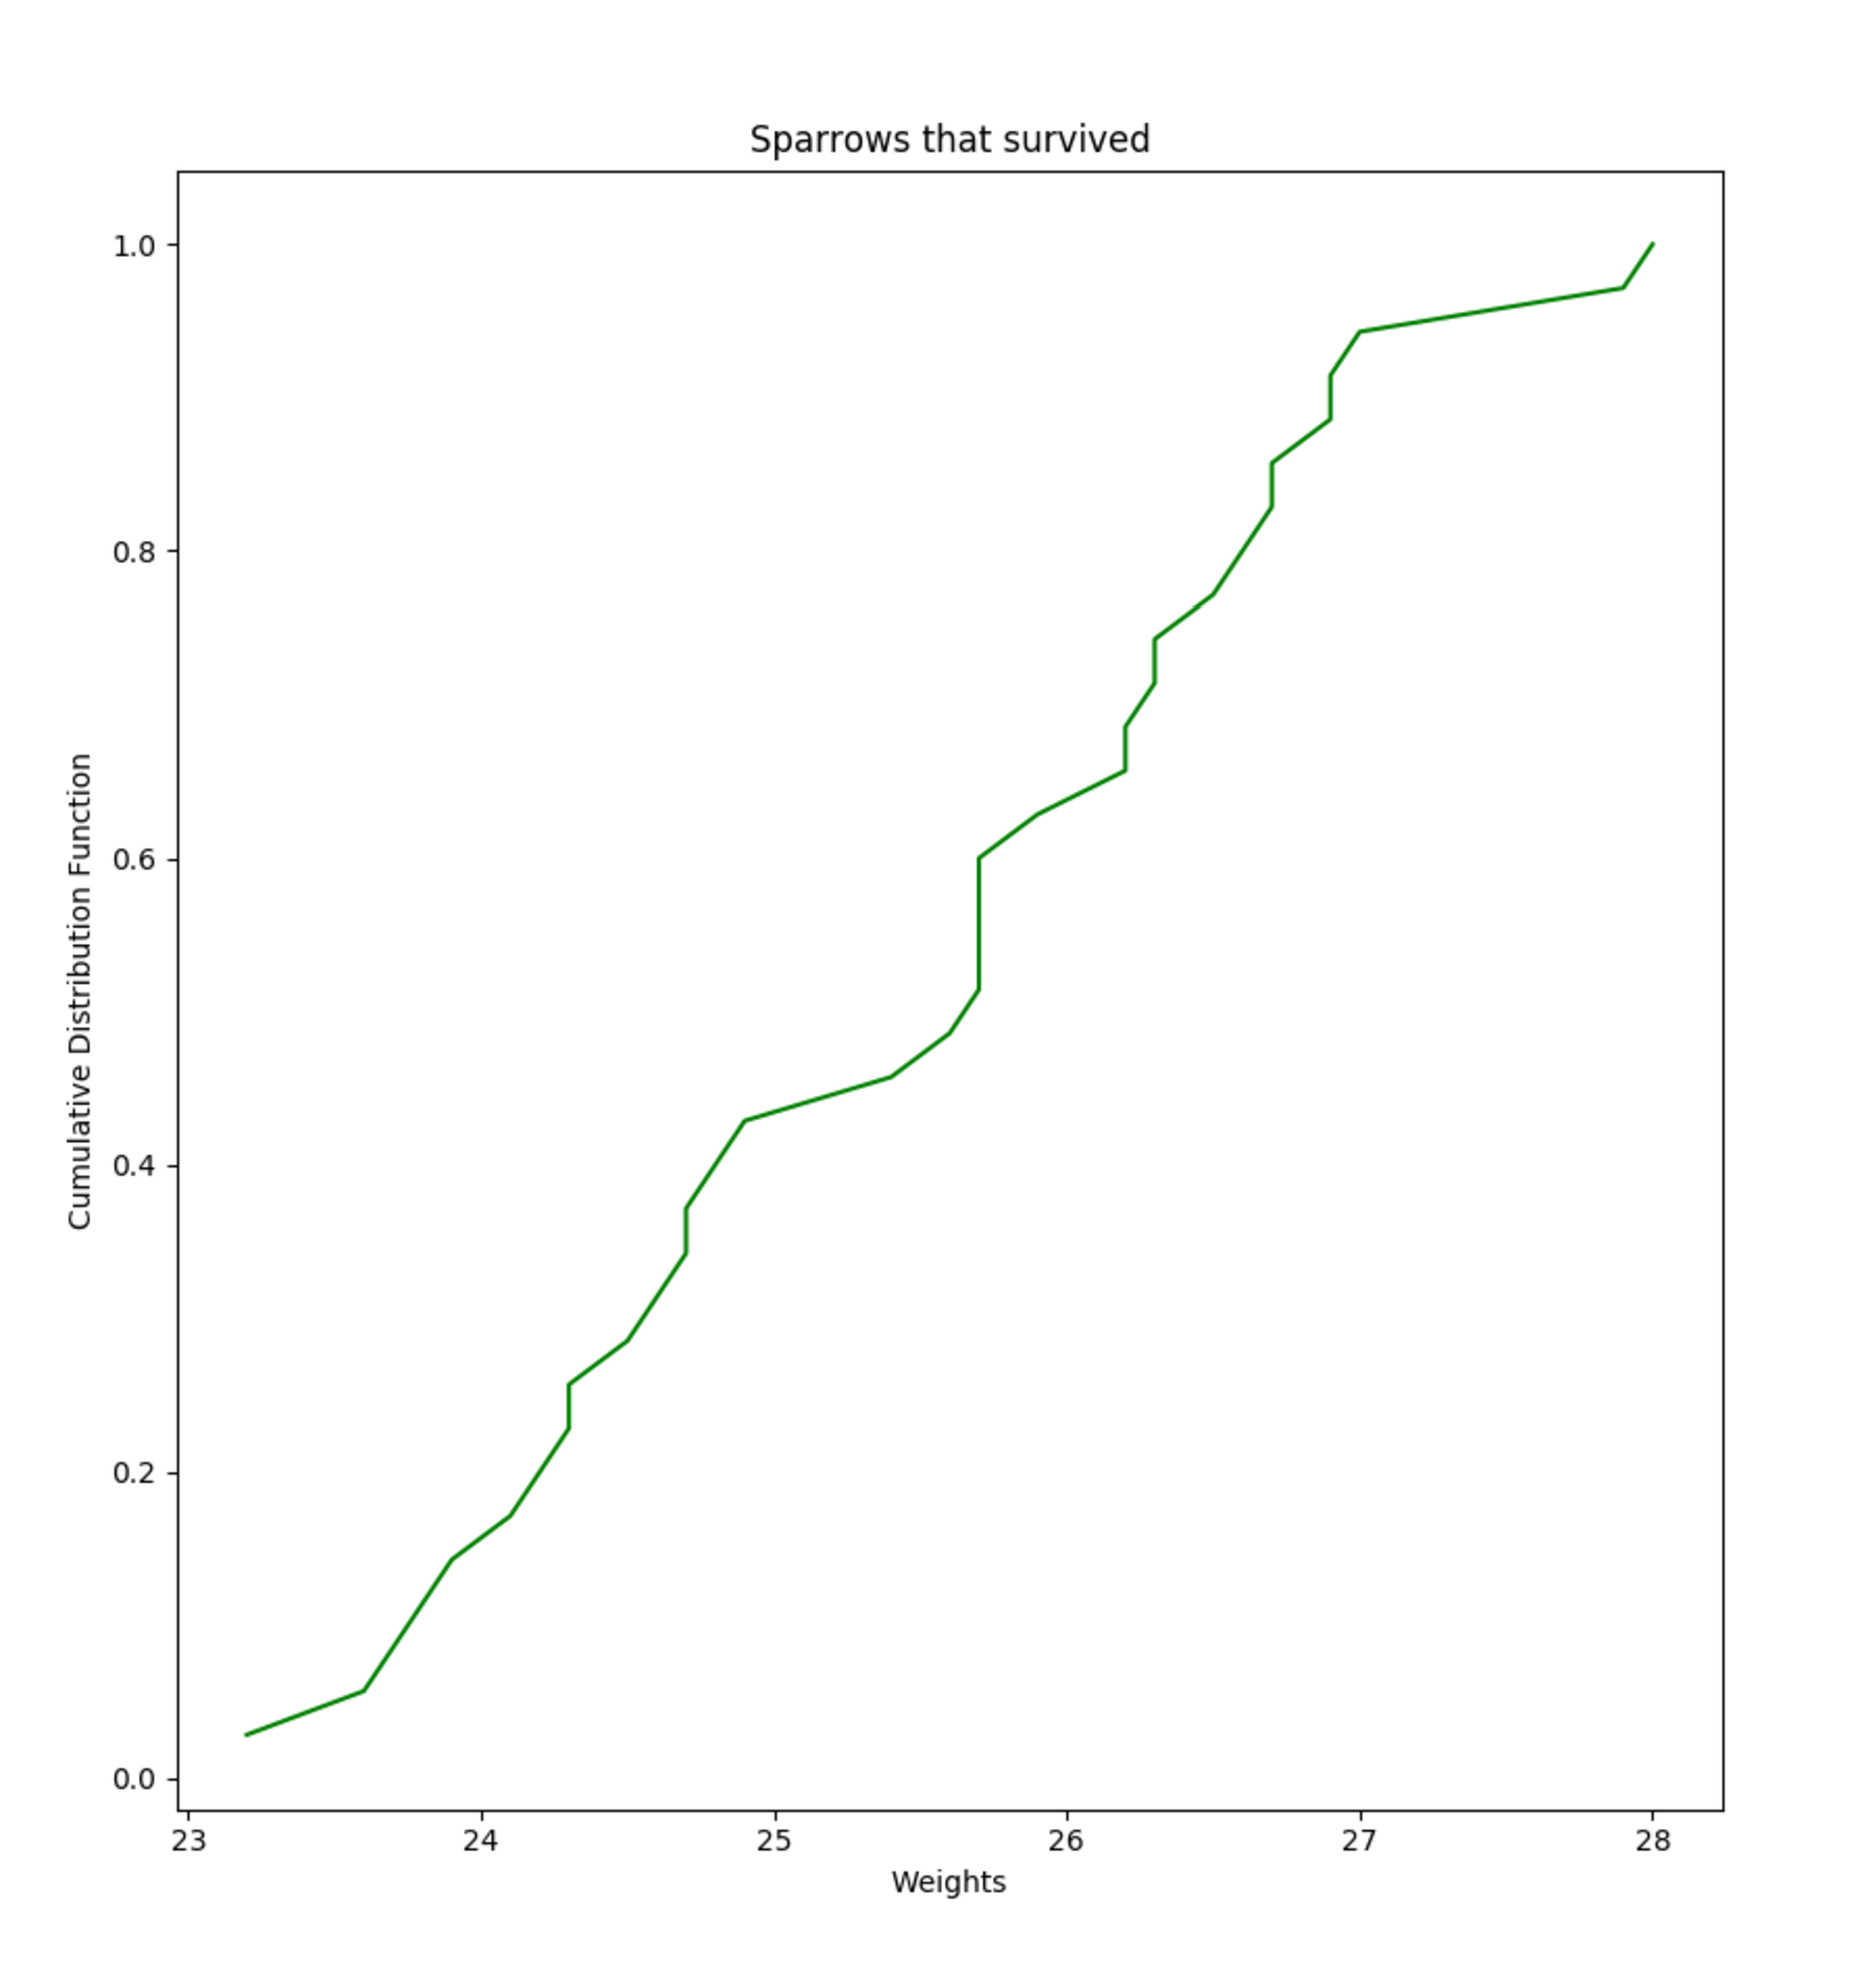
\includegraphics[height=3.5in]{survivedDist}

TODO.\par \bigskip

Poté vykreslíme histogram a graf empirické distribuční funkce pro vrabce kteří nepřežili.
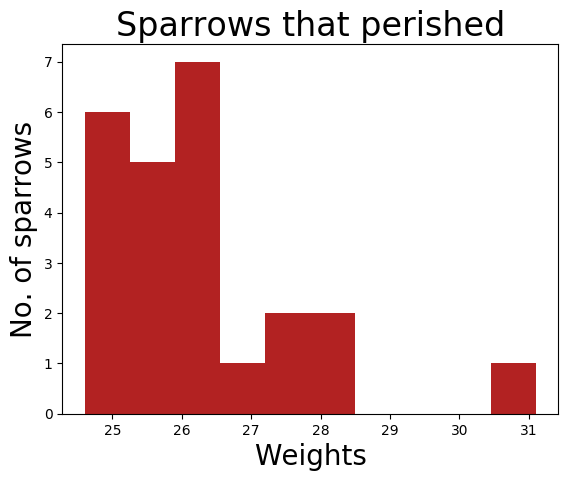
\includegraphics[height=3.5in]{diedHist}
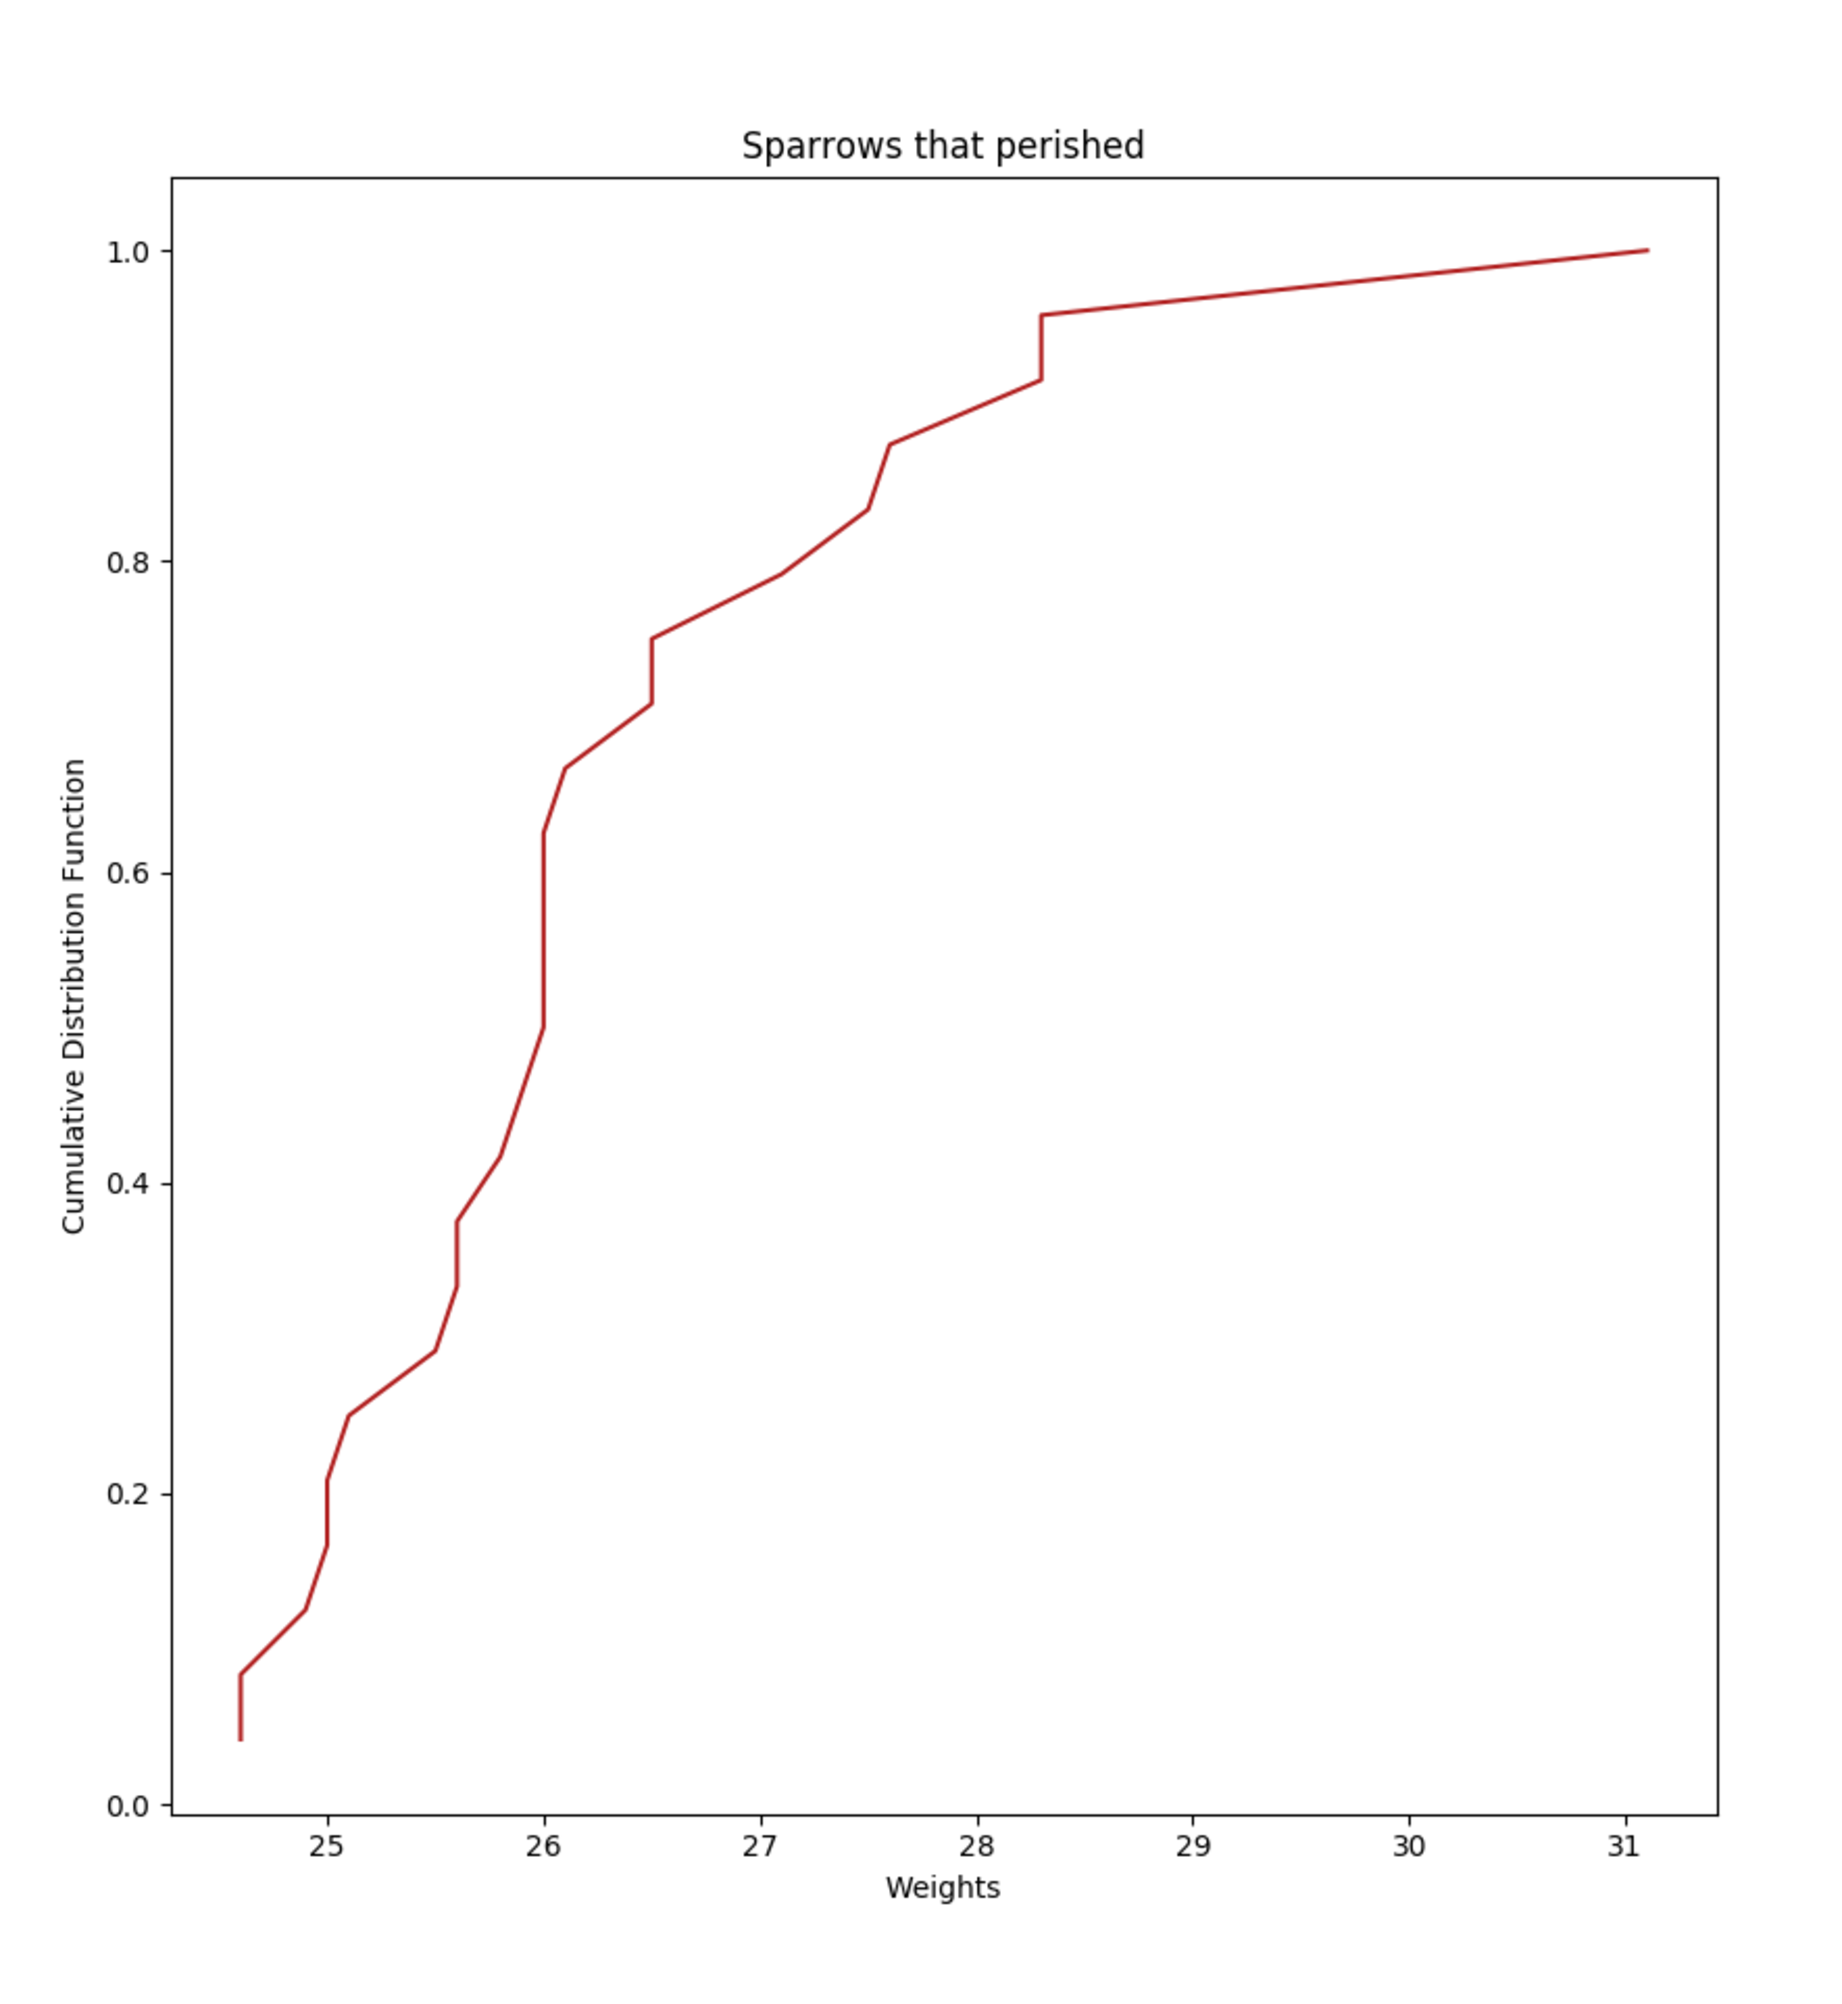
\includegraphics[height=3.5in]{diedDist}
Graf empirické distribuční funkce se podobá grafu exponenciálního rozdělení s parametrem $\lambda$ = 1.\par \bigskip

\section{Úkol 3}
\begin{center}
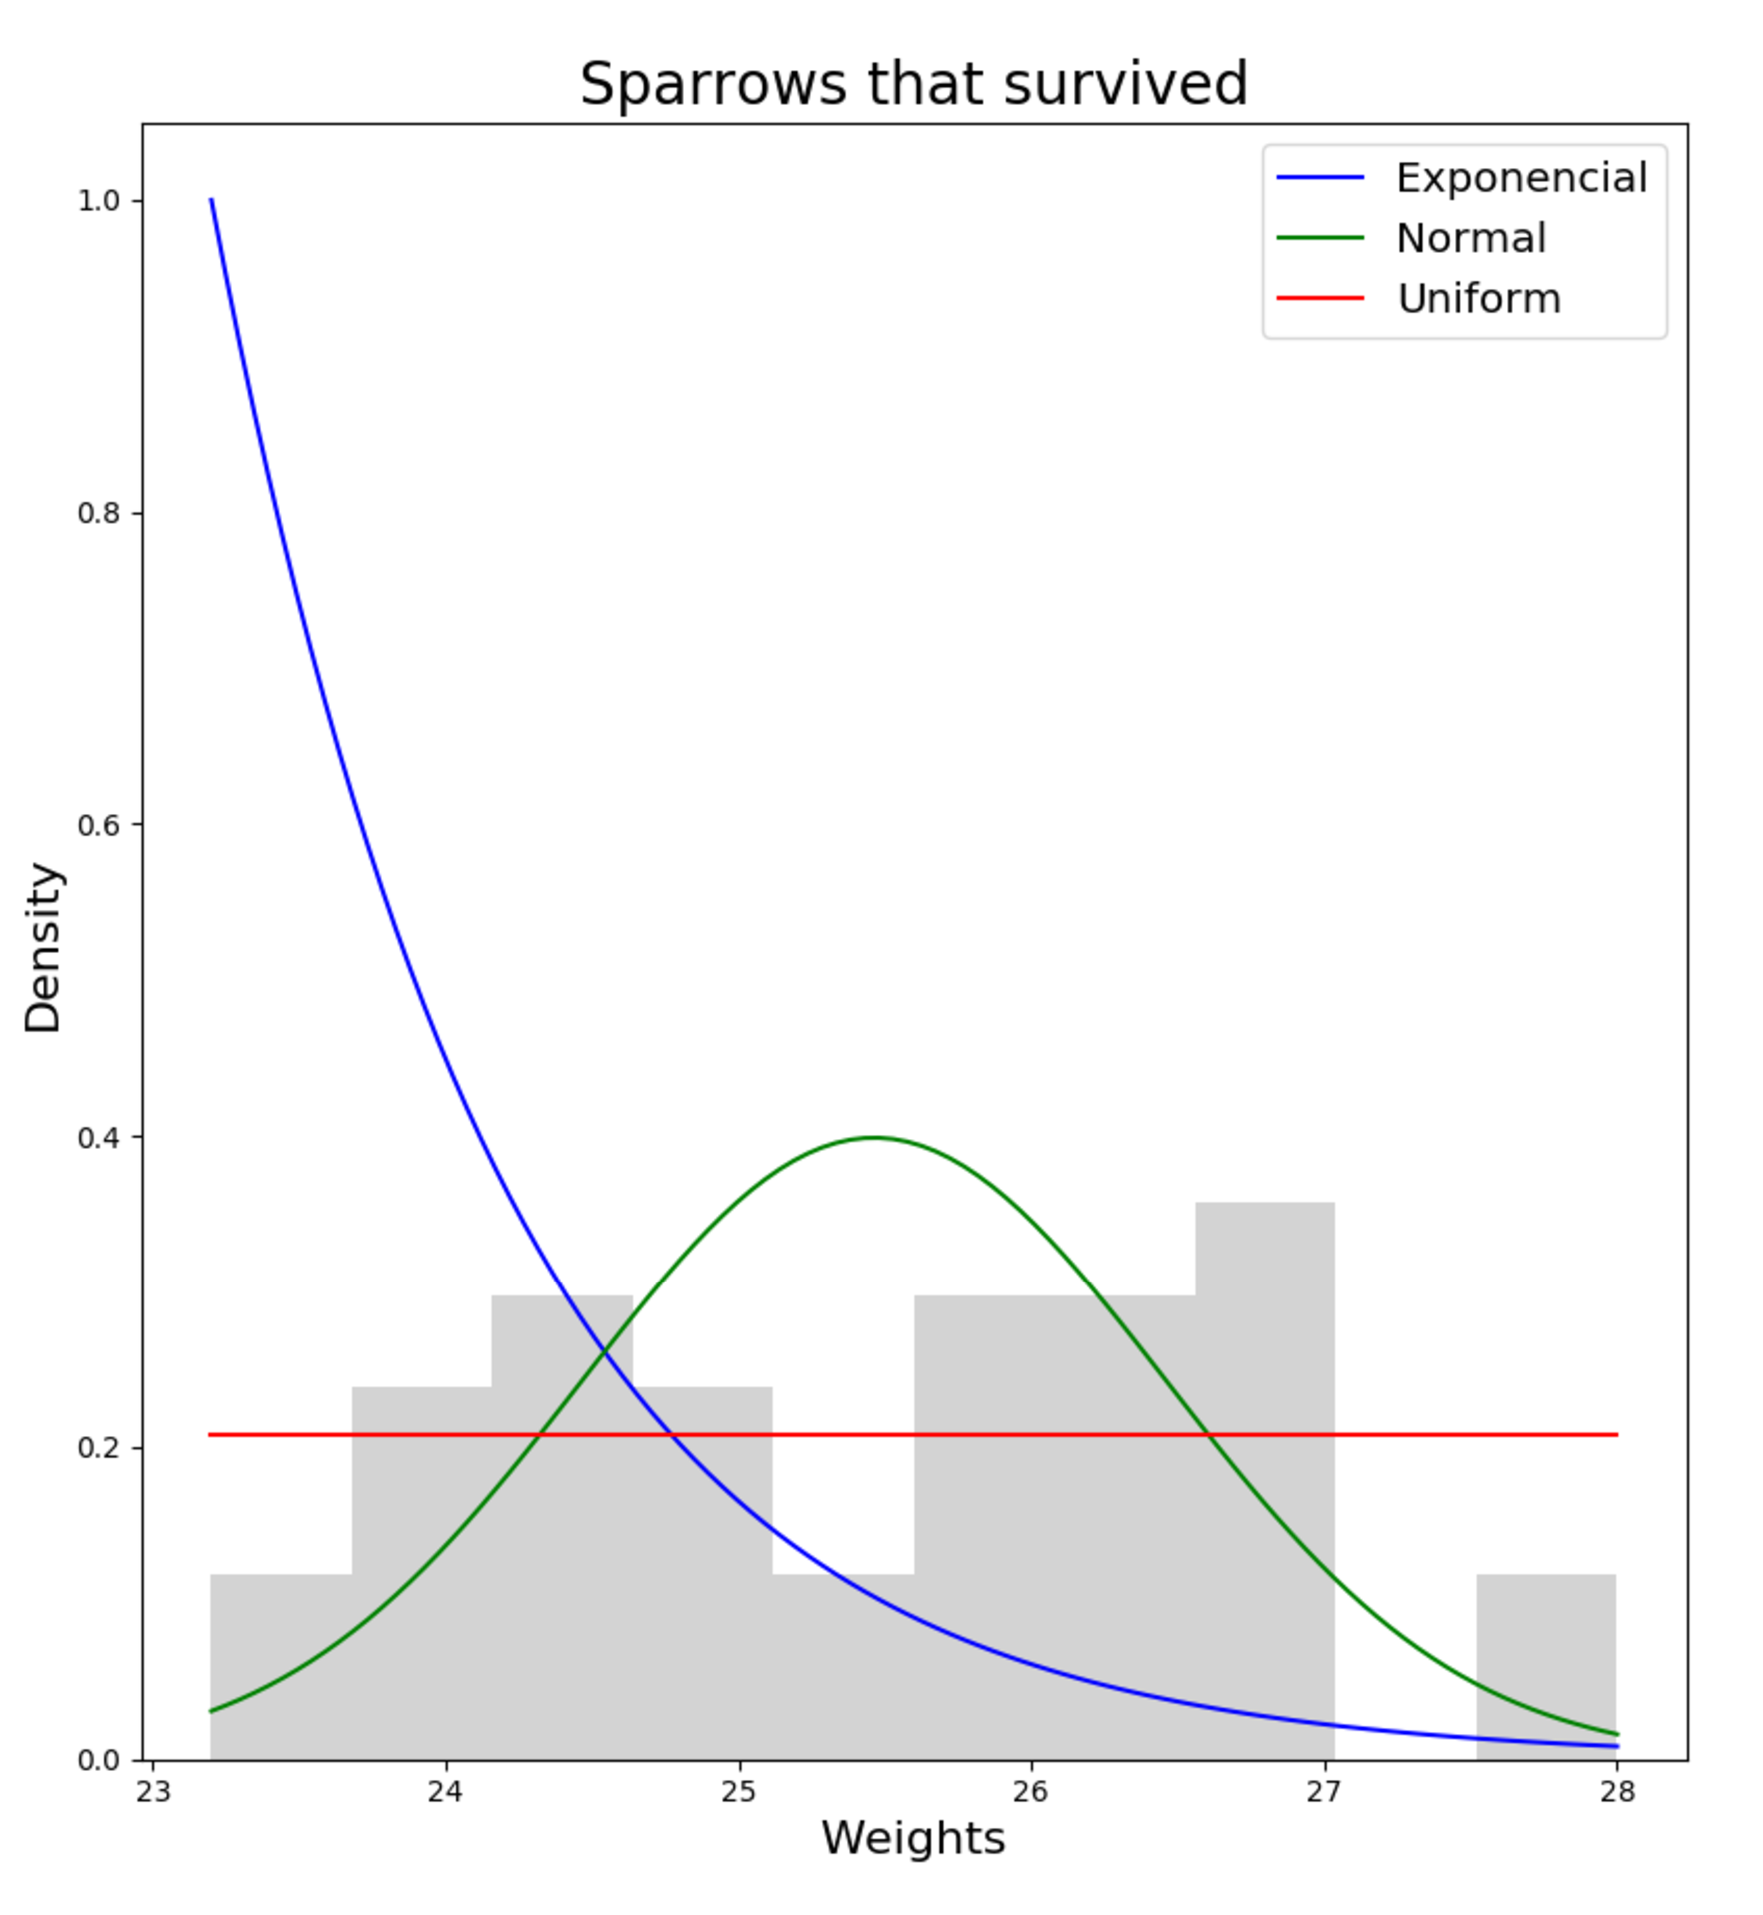
\includegraphics[width=5in]{3_survived}
\end{center}
\begin{center}
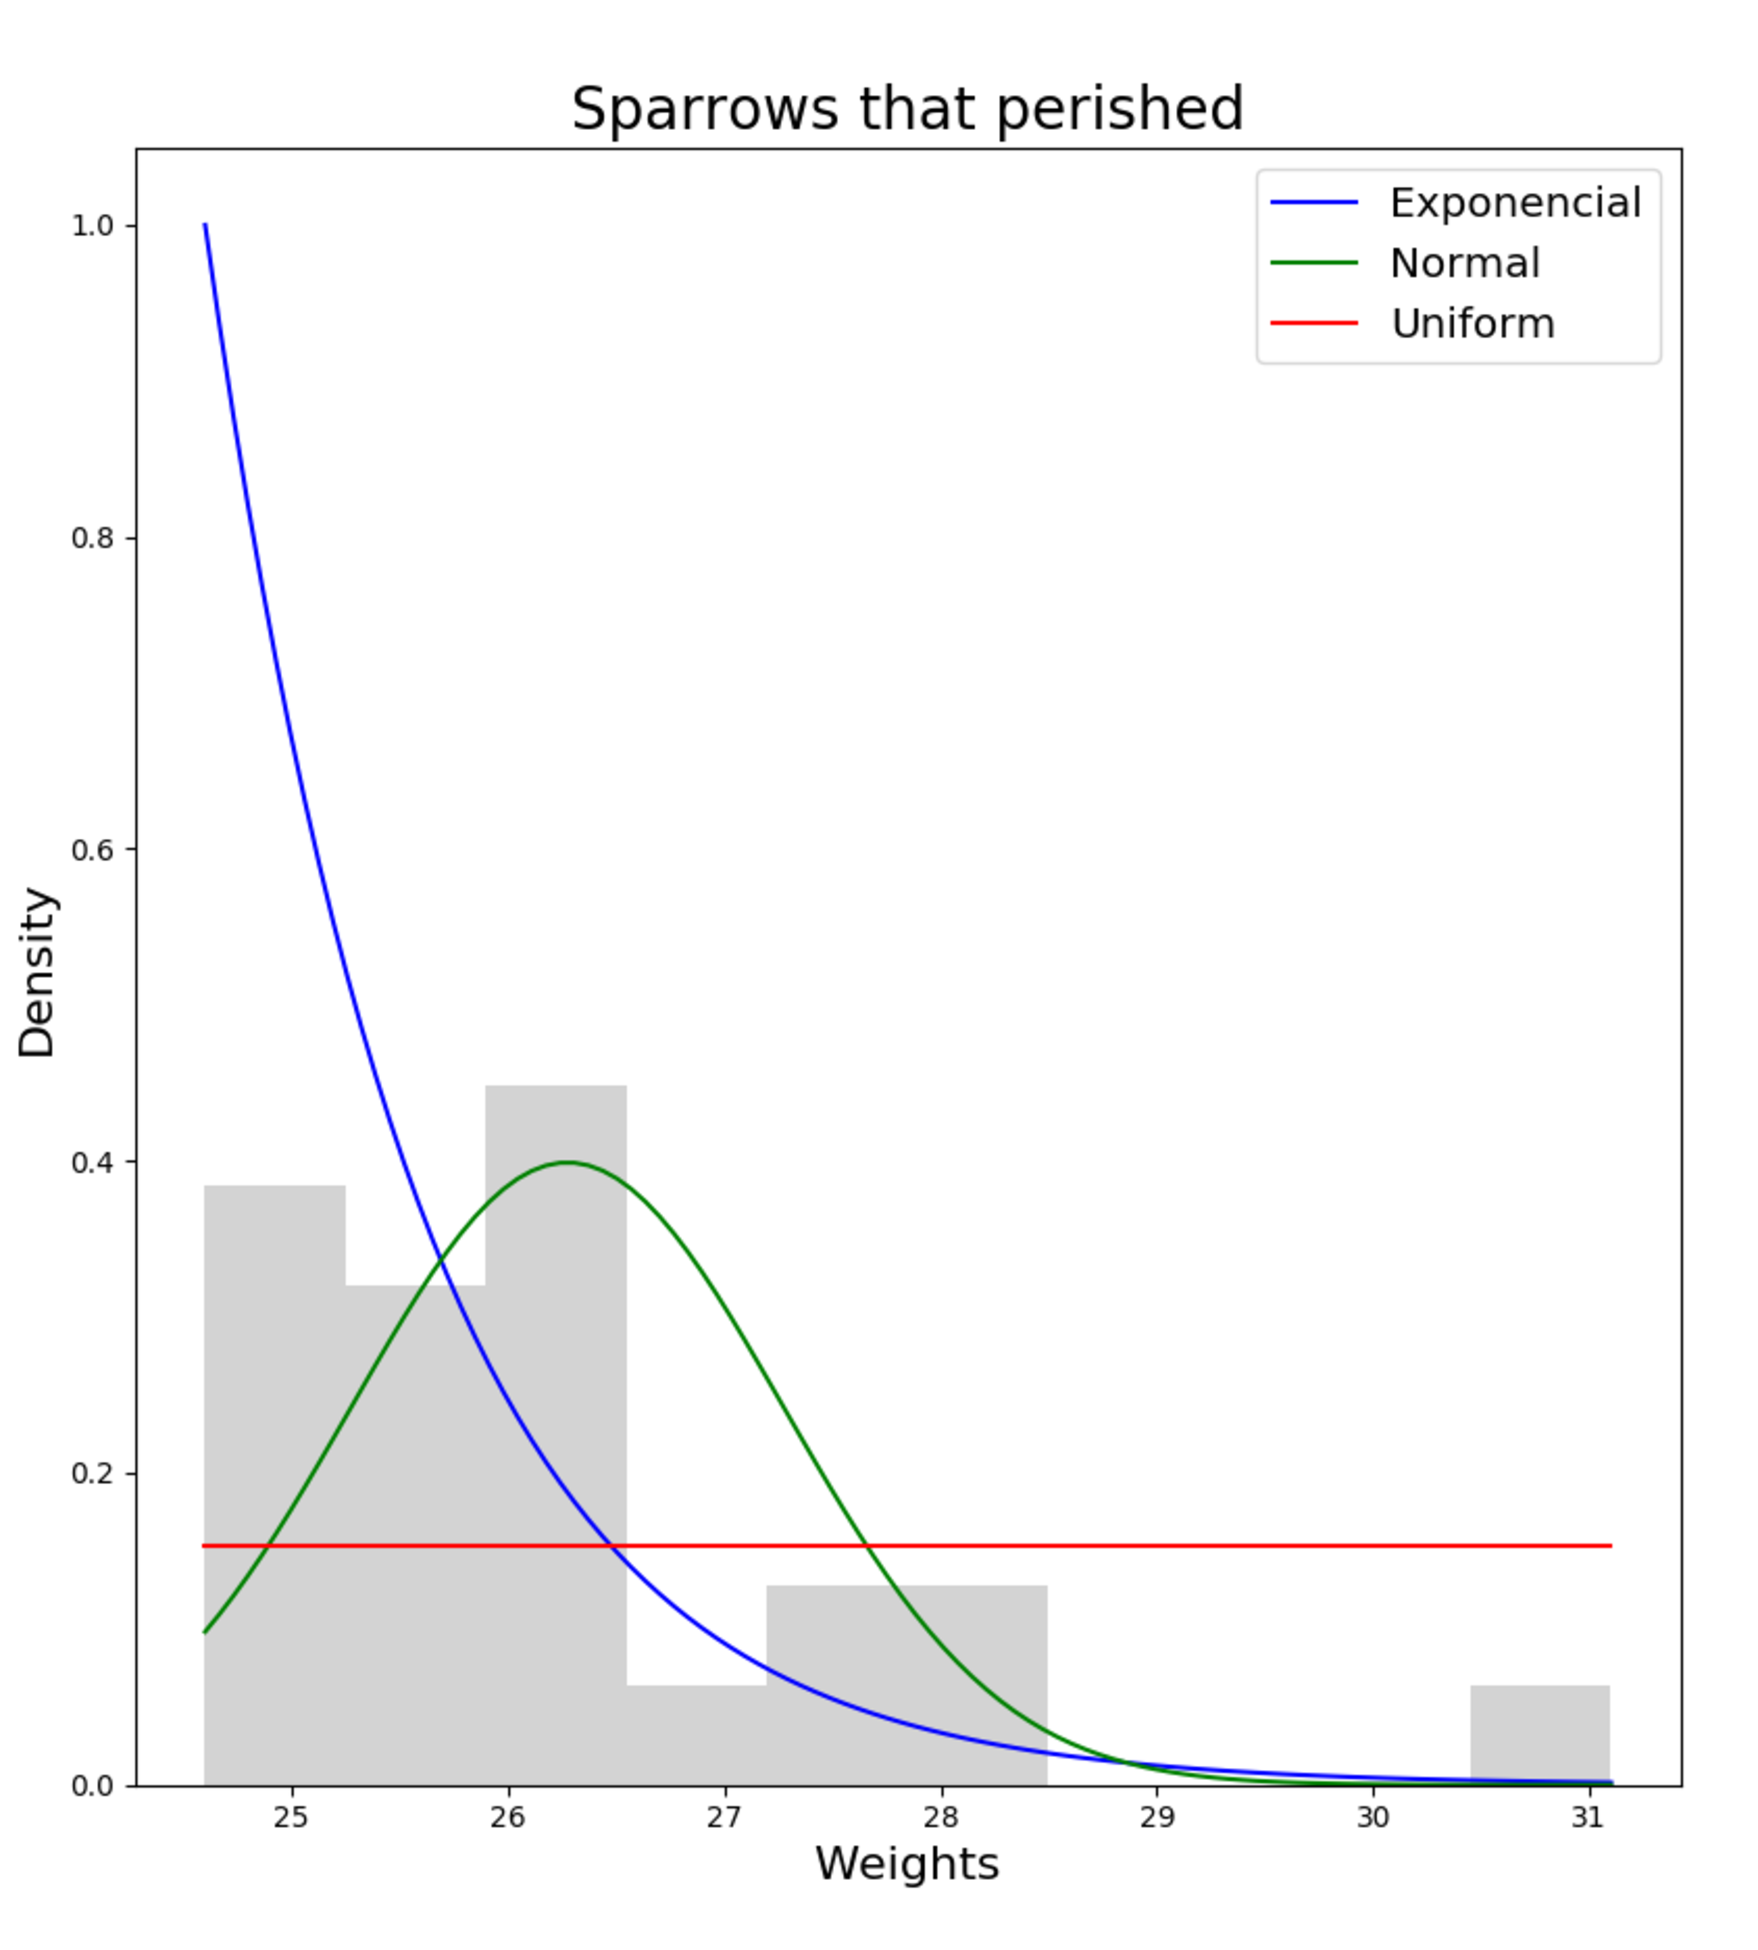
\includegraphics[width=5in]{3_died}
\end{center}

\section{Úkol 4}
Na následujících grafech je zobrazeno 100 vygenerovaných hodnot spolu s načtenými daty z datasetu. Histogram přeživších opeřenců vypadá jako normálního rozdělení s parametry $\lambda$ = EX = 25.793 a $\sigma ^2$ = varX = 1.918, hodnoty byli tedy generovány s těmito parametry. 

První graf vygenerovaných dat poměrně silně připomíná získaná data, věříme tedy že toto rozdělení bylo zvoleno správně.

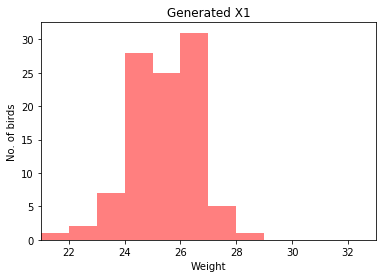
\includegraphics[width=3.2in]{4_Survived_Gen}
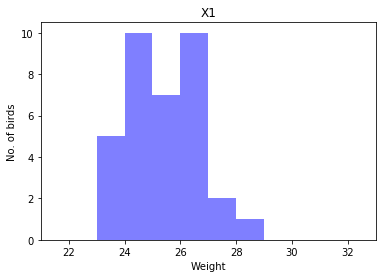
\includegraphics[width=3.2in]{4_Survived_Data}

Data vygenerovaná pro mrtvé opeřence už na tom nejsou tak dobře, část dat "utíká" do strany, zde by se hodilo mít větší dataset aby se dala lépe odhadnout distribuční funkce, popřípadě lépe vystihnout parametry rozdělení.

Pro opeřence jež nepřežili byla data generována s normální distribuční funkcí s parametry $\lambda$ = EX = 26.275 a $\sigma ^2$ = varX = 2.078.

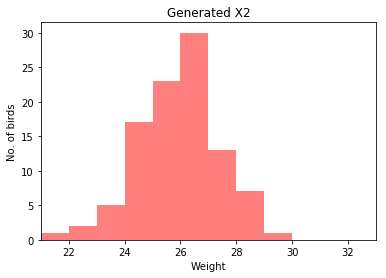
\includegraphics[width=3.2in]{4_Died_Gen}
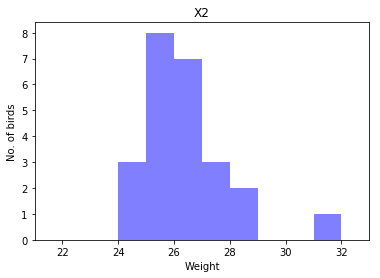
\includegraphics[width=3.2in]{4_Died_Data}

\par \bigskip

\section{Úkol 5}

$\bar{X}_n$ je výběrový průměr veličiny, $\sigma$ je směrodatná odchylka, n je počet prvků v rozdělení. Spolehlivost má být 95\%, tedy 
\begin{align*}
\alpha = 0.05 \Rightarrow \alpha/2 = 0.025 \\
z_{a/2} = z_{0,025} = \Phi^{-1}(0.975) \doteq 1.96
\end{align*}

Oboustranný 95\% konfidenční interval spočteme jako:

\begin{align}
(S_{X1},U_{X1}) = (\overbar{X1}_n - z_{a/2}.\frac{\sigma_1}{\sqrt{n_1}}, \overbar{X1}_n + z_{a/2}.\frac{\sigma_1}{\sqrt{n_1}}) \nonumber\\
= (25,463 - 1,96.\frac{1,24}{5,9}, 25,463 + 1,96.\frac{1,24}{5,9}) = (25.052, 25.874)
\end{align}

\begin{align}
(S_{X2},U_{X2}) = (\overbar{X2}_n - z_{a/2}.\frac{\sigma_2}{\sqrt{n_2}}, \overbar{X2}_n + z_{a/2}.\frac{\sigma_2}{\sqrt{n_2}}) \nonumber\\
= (26.275 - 1,96.\frac{1,44}{4,9}, 26.275 + 1,96.\frac{1,44}{4,9}) = (25.698, 26.852)
\end{align}



\end{document}

